 \documentclass[25pt, a0paper, portrait, margin=0mm, innermargin=15mm,
     blockverticalspace=15mm, colspace=15mm, subcolspace=8mm]{tikzposter} %Default values for poster format options.
     
\usepackage{tabularx,booktabs,adjustbox} % For tables
\usepackage{wrapfig,anyfontsize,lipsum}
\linespread{1.2}
\usetikzlibrary{calc,fit,arrows,decorations.pathmorphing,backgrounds,fit,positioning,patterns}
\usetikzlibrary{shapes.symbols}

\usepackage{color,colortbl}
\definecolor{Cblack}{rgb}{0,0,0}
\definecolor{Corange}{rgb}{0.9,0.6,0}
\definecolor{Cskyblue}{rgb}{0.35,0.7,0.9}
\definecolor{Cbluegreen}{rgb}{0,0.6,0.5}
\definecolor{Cyellow}{rgb}{0.95,0.9,0.25}
\definecolor{Cblue}{rgb}{0,0.45,0.7}
\definecolor{Cvermillion}{rgb}{0.8,0.4,0}
\definecolor{Cpurple}{rgb}{0.8,0.6,0.7}

\newcommand{\Cblack}[1]{\textcolor{Cblack}{#1}}
\newcommand{\Corange}[1]{\textcolor{Corange}{#1}}
\newcommand{\Cskyblue}[1]{\textcolor{Cskyblue}{#1}}
\newcommand{\Cbluegreen}[1]{\textcolor{Cbluegreen}{#1}}
\newcommand{\Cyellow}[1]{\textcolor{Cyellow}{#1}}
\newcommand{\Cblue}[1]{\textcolor{Cblue}{#1}}
\newcommand{\Cvermillion}[1]{\textcolor{Cvermillion}{#1}}
\newcommand{\Cpurple}[1]{\textcolor{Cpurple}{#1}}

 \newcommand{\magenta}[1]{\textcolor{magenta}{#1}}
 \newcommand{\teal}[1]{\textcolor{teal}{#1}}
  \newcommand{\gray}[1]{\textcolor{gray}{#1}}

% tikz colour settings
\tikzset{pop0/.style={red!50!yellow},pop1/.style={violet!80},pop2/.style={olive!70!green}}

\definecolorpalette{myColorPalette} {
\definecolor{colorOne}{named}{teal}
\definecolor{colorTwo}{named}{white}
\definecolor{colorThree}{named}{cyan}
}

 \tikzposterlatexaffectionproofoff %shows small comment on how the poster was made at bottom of poster

 % Commands
 \newcommand{\bs}{\textbackslash}   % backslash
 \newcommand{\cmd}[1]{{\bf \color{red}#1}}   % highlights command
% \newcommand{\crossmark}{\ding{55}}

 % Title, Author, Institute
 \title{{\bf Analysis, inference and simulation of identity-by-descent in large datasets}}
 \author{{\bf Georgia Tsambos}}
 \institute{{\bf University of Melbourne, Australia}}

 % -- PREDEFINED THEMES ---------------------- %
 % Choose LAYOUT:  Default, Basic, Rays, Simple, Envelope, Wave, Board, Autumn, Desert,
 \usetheme{Autumn}
\usecolorstyle[colorPalette=myColorPalette]{Denmark}


 \begin{document}

     \maketitle
\block[bodyverticalshift=-2cm]{}{
   {\large\teal{
 Georgia Tsambos (1, 2), Peter Ralph (3), Jerome Kelleher (4), Stephen Leslie (1, 2, 5), Damjan Vukcevic (1, 2).
(1) School of Mathematics and Statistics, University of Melbourne, Australia (2) Melbourne Integrative Genomics, University of Melbourne, Australia, (3) Department of Mathematics, University of Oregon, United States, (4) Big Data Institute, University of Oxford, United Kingdom, (5) School of Biosciences, University of Melbourne, Australia. Presenting author: gtsambos (at) student.unimelb.edu.au}
}
}
   
   %%% BLOCK 0  
 \block[titleoffsety=1cm,bodyverticalshift=-20cm]{0. Introduction}{
 }
 \begin{columns}
 \begin{subcolumns}
   \subcolumn{31} \block[bodyoffsetx=1.5cm,bodyverticalshift=-5cm]{}{
{\fontsize{34}{35}\selectfont Identity-by-descent (IBD) analyses make it possible to study the relatedness of individuals on a detailed scale without invoking murky concepts of population labels. 
This poster showcases a recent advance in the tskit [1] software, the \texttt{find-ibd} method, which allows complete IBD information to be calculated efficiently on large samples at all time scales. 
The utility of this tool will be demonstrated with simulations, as well as with data from the Human Genome Diversity Project.}\\[3mm] 
    }
 \end{subcolumns}
 \end{columns}

%%% BLOCK 1
     \begin{columns}%blocks will be placed into columns
         \column{.5}
         \block[roundedcorners=40,titleoffsety=-3cm,bodyoffsety=-3cm,bodyverticalshift=-1cm]{1. Data structures and definitions}{

{\fontsize{34}{35}\selectfont The {\bf\magenta{tree sequence}} data structure [1,2] encodes a complete genealogy for a sample of chromosomes in a succinct set of tables. Compared with traditional sequence-based formats, tree sequences are \emph{compact}, \emph{fast} to process and \emph{informative} of the history of the sample.

\vspace{10mm}

\begin{center}

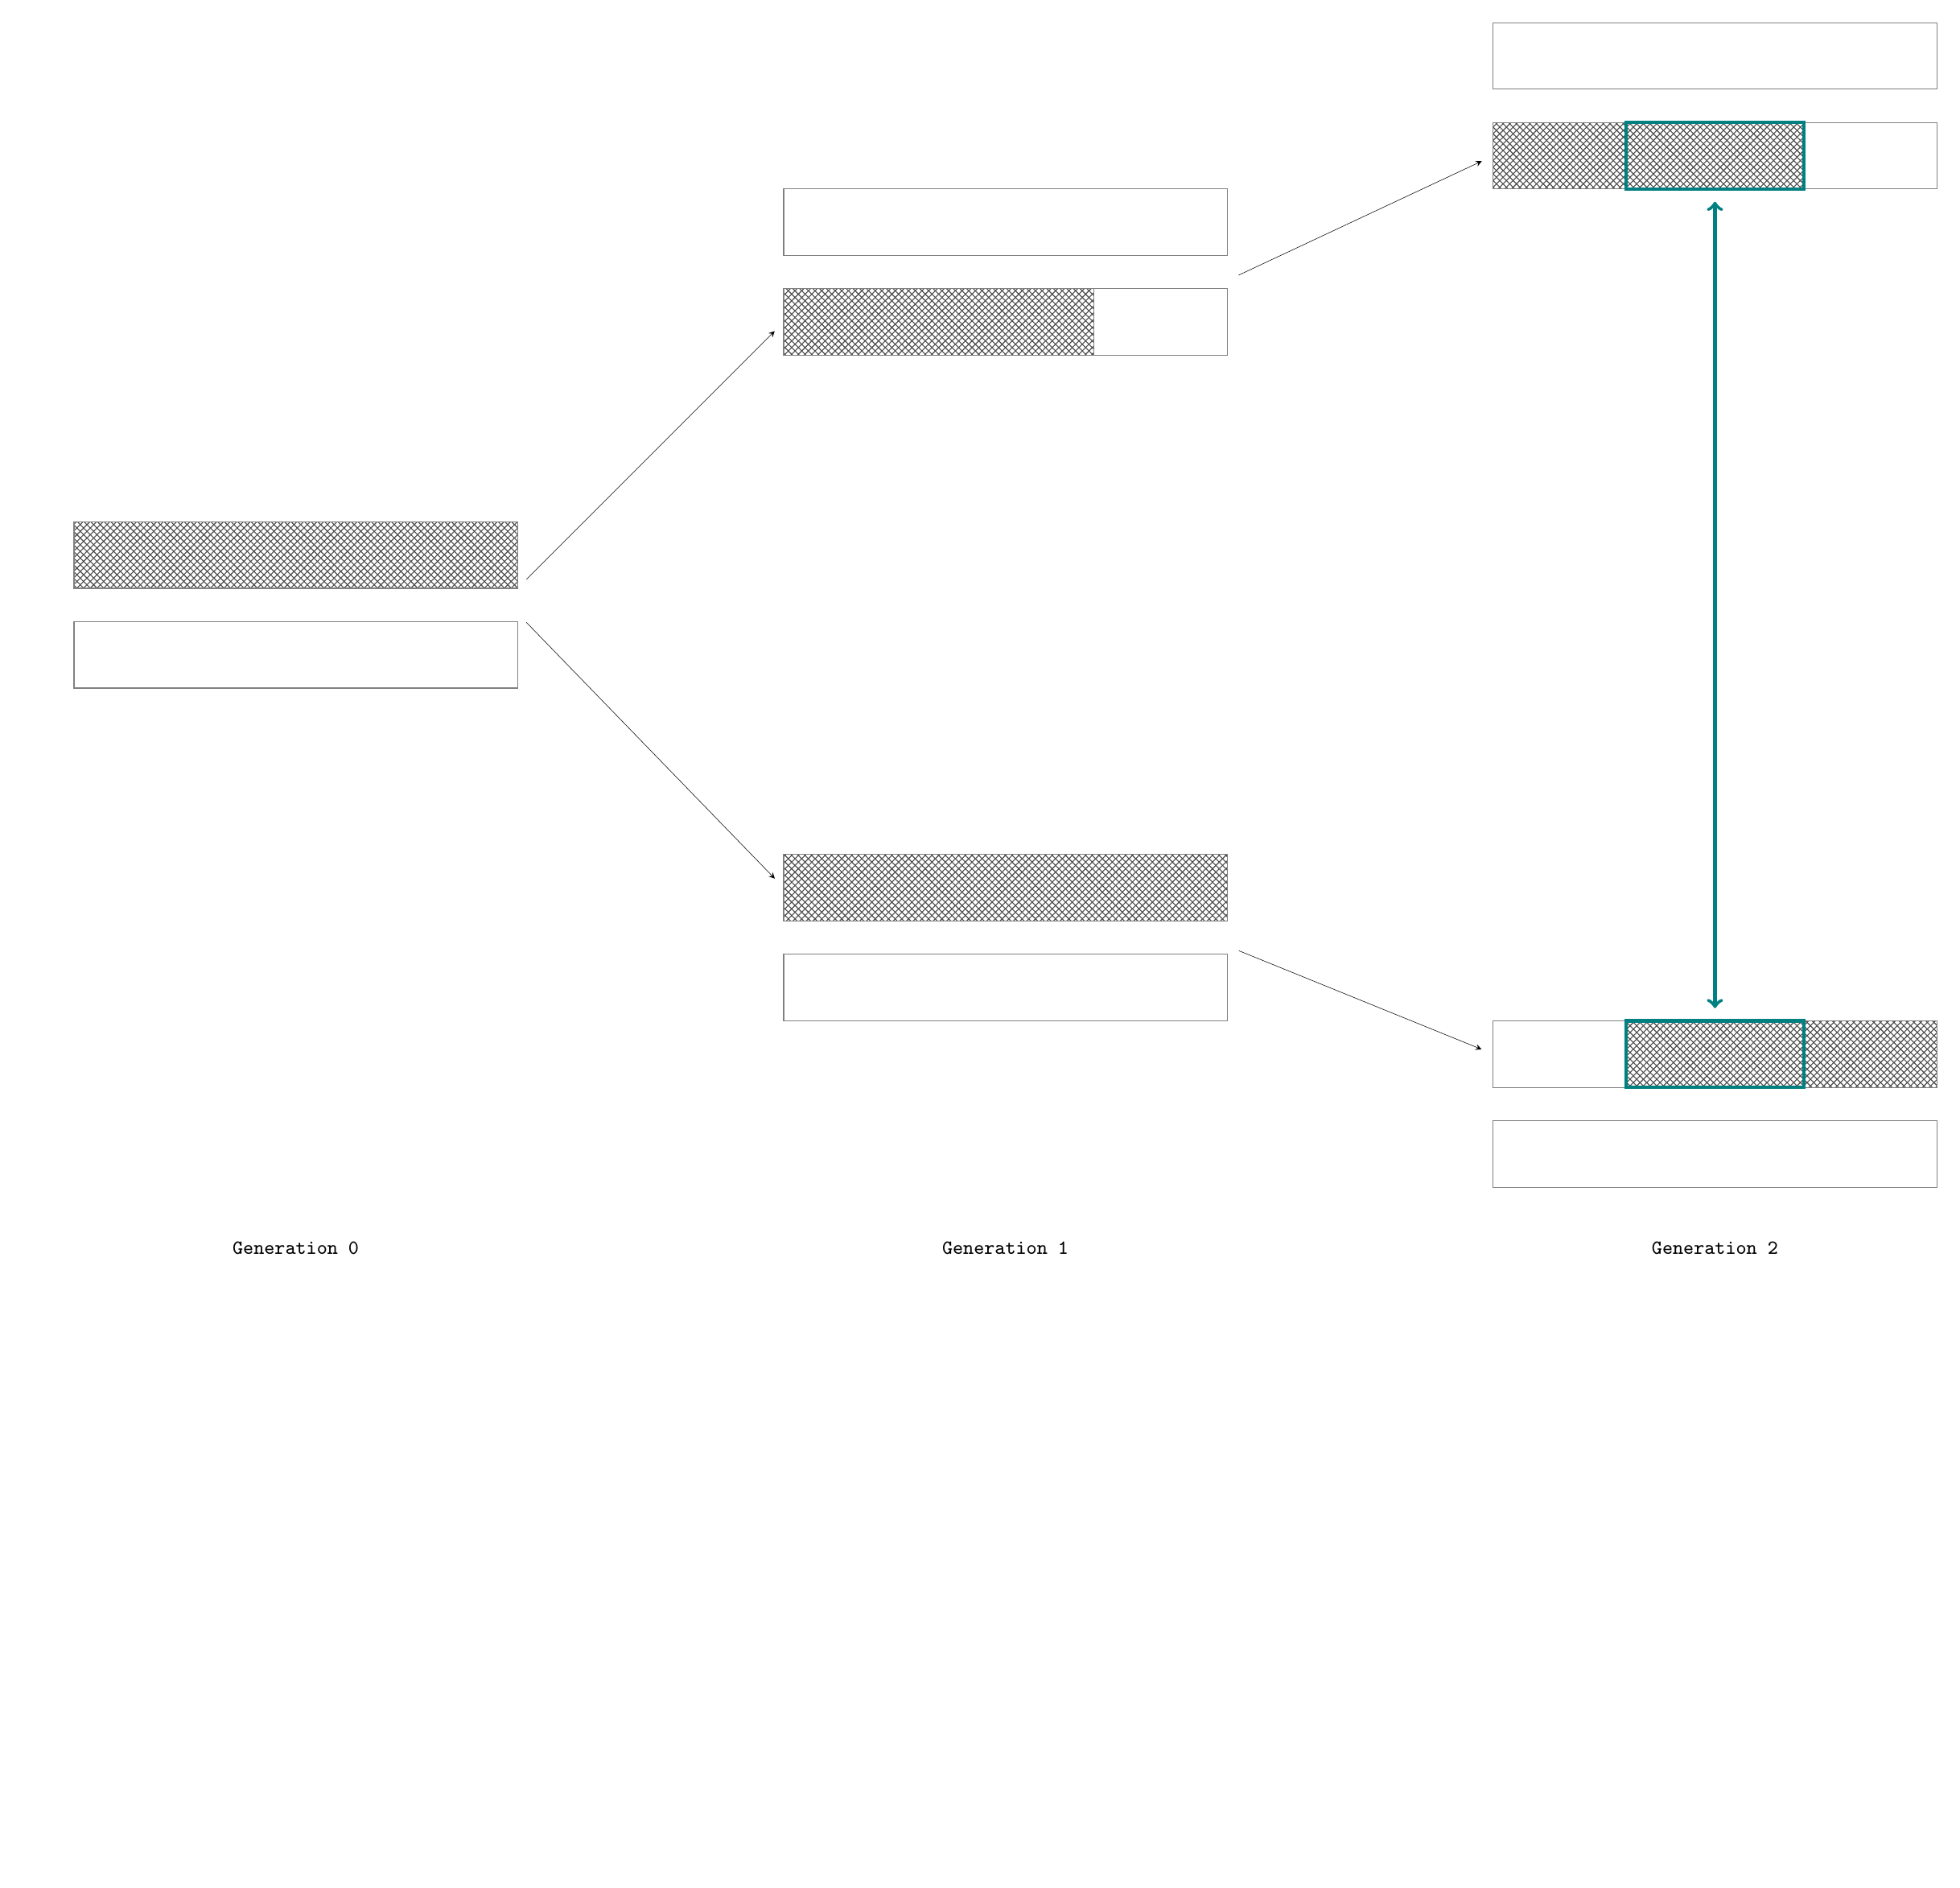
\begin{tikzpicture}[yscale=0.7, xscale=0.7]

\tikzset{
pop1/.style={fill=blue!40,draw=black!50},
pop2/.style={fill=red!40,draw=black!50},
ibd/.style={pattern=crosshatch,pattern color=black!70,draw=black!50},
nonibd/.style={fill=white,draw=black!50},
inherit/.style={->,>=stealth,thick,shorten <=2mm,shorten >=2mm,very thin},
recomb/.style={thick,draw=black!70}
}

% Nodes
\node (hapx) at (1,0) {};
\node (hapy) at (0,1.5) {};
\node (hapxy) at ($10*(hapx) + (hapy)$) {};

\node (gen1) at (0,0) {};
\node (gen2) at ($8*(hapx) + 0*(hapx)$) {};
\node (gen3) at ($8*(hapx) + 8*(hapx)$) {};

\node (ind1gen3) at ($(gen3) + (0,0)$) {};
\node (indsep) at ($5*(hapy)$) {};

\node (ind1gen2) at ($(gen2) + 1*(indsep)$) {};
\node (ind2gen2) at ($(gen2) - 1*(indsep)$) {};

\node (ind1gen1) at ($(gen1) + 1.5*(indsep)$) {};
\node (ind2gen1) at ($(gen1) + 0.5*(indsep)$) {};
\node (ind3gen1) at ($(gen1) - 0.5*(indsep)$) {};
\node (ind4gen1) at ($(gen1) - 1.5*(indsep)$) {};

\node (chr1) at ($0.25*(hapy)$)  {};
\node (chr2) at ($-1.25*(hapy)$) {};


%% Haplotypes
%
%\filldraw[pop1] ($(gen1) + (ind1gen1) + (chr1)$) rectangle +(hapxy);
%\filldraw[pop1] ($(gen1) + (ind1gen1) + (chr2)$) rectangle +(hapxy);
%
%\filldraw[pop2] ($(gen1) + (ind2gen1) + (chr1)$) rectangle +(hapxy);
%\filldraw[pop2] ($(gen1) + (ind2gen1) + (chr2)$) rectangle +(hapxy);
%
%\filldraw[pop1] ($(gen1) + (ind3gen1) + (chr1)$) rectangle +(hapxy);
%\filldraw[pop1] ($(gen1) + (ind3gen1) + (chr2)$) rectangle +(hapxy);
%
%\filldraw[pop2] ($(gen1) + (ind4gen1) + (chr1)$) rectangle +(hapxy);
%\filldraw[pop2] ($(gen1) + (ind4gen1) + (chr2)$) rectangle +(hapxy);
%
%
%\filldraw[pop1] ($(gen2) + (ind1gen2) + (chr1)$) rectangle +(hapxy);
%\filldraw[pop2] ($(gen2) + (ind1gen2) + (chr2)$) rectangle +(hapxy);
%
%\filldraw[pop1] ($(gen2) + (ind2gen2) + (chr1)$) rectangle +(hapxy);
%\filldraw[pop2] ($(gen2) + (ind2gen2) + (chr2)$) rectangle +(hapxy);
%
%
%\filldraw[pop1] ($(gen3) + (ind1gen3) + (chr1)$) rectangle +(hapxy);
%\fill[pop1] ($(gen3) + (ind1gen3) + (chr2)$) rectangle +(hapxy);
%\fill[pop2] ($(gen3) + (ind1gen3) + (chr2)+ 2*(hapx)$) rectangle ($(gen3) + (ind1gen3) + (chr2)+ (hapxy)$);
%\fill[pop1] ($(gen3) + (ind1gen3) + (chr2)+ 4*(hapx)$) rectangle ($(gen3) + (ind1gen3) + (chr2)+ (hapxy)$);
%\fill[pop2] ($(gen3) + (ind1gen3) + (chr2)+ 9*(hapx)$) rectangle ($(gen3) + (ind1gen3) + (chr2)+ (hapxy)$);
%%\draw ($(gen3) + (ind1gen3) + (chr2)$) rectangle +(hapxy);
%
%
%% Copying lines
%
\node (startline) at ($-1*(hapx) + 0.5*(hapy)$) {};
\node (chrdiff) at ($(chr1) - (chr2)$) {};
%
%
%% Arrows
%\draw[inherit] ($(gen1) + (ind1gen1) + (chr2) + 10*(hapx) + 0.75*(chrdiff)$) -- ($(gen2) + (ind1gen2) + (chr1) + 0.5*(hapy)$);
%\draw[inherit] ($(gen1) + (ind2gen1) + (chr2) + 10*(hapx) + 0.75*(chrdiff)$) -- ($(gen2) + (ind1gen2) + (chr2) + 0.5*(hapy)$);
%\draw[inherit] ($(gen1) + (ind3gen1) + (chr2) + 10*(hapx) + 0.75*(chrdiff)$) -- ($(gen2) + (ind2gen2) + (chr1) + 0.5*(hapy)$);
%\draw[inherit] ($(gen1) + (ind4gen1) + (chr2) + 10*(hapx) + 0.75*(chrdiff)$) -- ($(gen2) + (ind2gen2) + (chr2) + 0.5*(hapy)$);
%
%\draw[inherit] ($(gen2) + (ind1gen2) + (chr2) + 10*(hapx) + 0.75*(chrdiff)$) -- ($(gen3) + (ind1gen3) + (chr1) + 0.5*(hapy)$);
%\draw[inherit] ($(gen2) + (ind2gen2) + (chr2) + 10*(hapx) + 0.75*(chrdiff)$) -- ($(gen3) + (ind1gen3) + (chr2) + 0.5*(hapy)$);


%%%%%%%%%%%%%%%%%%%%%
% Identity-by-descent
% Nodes
\node (hapx) at (1,0) {};
\node (hapyIBD) at (0,+17.0) {};
%\node (hapxy) at ($10*(hapx) + (hapy)$) {};

%\node (gen1) at (0,0) {};
%\node (gen2) at ($8*(hapx) + 0*(hapx)$) {};
%\node (gen3) at ($8*(hapx) + 8*(hapx)$) {};

%\node (indsep) at ($5*(hapy)$) {};
\node (ind1gen3) at ($(gen3) + 1.5*(indsep)$) {};
\node (ind2gen3) at ($(gen3) - 1.5*(indsep)$) {};

\node (ind1gen2) at ($(gen2) + 1*(indsep)$) {};
\node (ind2gen2) at ($(gen2) - 1*(indsep)$) {};

\node (ind1gen1) at ($(gen1) + 0*(indsep)$) {};

\node (chr1) at ($0.25*(hapy) + (hapyIBD)$)  {};
\node (chr2) at ($-1.25*(hapy)+ (hapyIBD)$) {};

% Haplotypes
\filldraw[ibd] ($(gen1) + (ind1gen1) + (chr1)$) rectangle +(hapxy);
\filldraw[nonibd] ($(gen1) + (ind1gen1) + (chr2)$) rectangle +(hapxy);

\filldraw[nonibd] ($(gen2) + (ind1gen2) + (chr1)$) rectangle +(hapxy);
\filldraw[ibd] ($(gen2) + (ind1gen2) + (chr2)$) rectangle +(hapxy);
\filldraw[nonibd] ($(gen2) + 7*(hapx) + (ind1gen2) + (chr2)$) rectangle ($(gen2) + (ind1gen2) + (chr2) + (hapxy)$);

\filldraw[ibd] ($(gen2) + (ind2gen2) + (chr1)$) rectangle +(hapxy);
%\filldraw[ibd] ($(gen2) + 3*(hapx) + (ind2gen2) + (chr1)$) rectangle ($(gen2) + (hapxy) + (ind2gen2) + (chr1)$);
\filldraw[nonibd] ($(gen2) + (ind2gen2) + (chr2)$) rectangle +(hapxy);

\filldraw[nonibd] ($(gen3) + (ind1gen3) + (chr1)$) rectangle +(hapxy);
\filldraw[ibd] ($(gen3) + (ind1gen3) + (chr2)$) rectangle +(hapxy);
\filldraw[nonibd] ($(gen3) + 7*(hapx) + (ind1gen3) + (chr2)$) rectangle ($(gen3) + (ind1gen3) + (chr2) + (hapxy)$);

\filldraw[nonibd] ($(gen3) + (ind2gen3) + (chr1)$) rectangle +(hapxy);
\filldraw[ibd] ($(gen3) + 3*(hapx) + (ind2gen3) + (chr1)$) rectangle ($(gen3) + (hapxy) + (ind2gen3) + (chr1)$);
\filldraw[nonibd] ($(gen3) + (ind2gen3) + (chr2)$) rectangle +(hapxy);

% Arrows
\draw[inherit] ($(gen1) + (ind1gen1) + (chr1) + 10*(hapx) + 0*(chrdiff)$) -- ($(gen2) + (ind1gen2) + (chr2) + 0.5*(hapy)$);
\draw[inherit] ($(gen1) + (ind1gen1) + (chr1) + 10*(hapx) - 0.25*(chrdiff)$) -- ($(gen2) + (ind2gen2) + (chr1) + 0.5*(hapy)$);

\draw[inherit] ($(gen2) + (ind1gen2) + (chr2) + 10*(hapx) + 0.75*(chrdiff)$) -- ($(gen3) + (ind1gen3) + (chr2) + 0.5*(hapy)$);
\draw[inherit] ($(gen2) + (ind2gen2) + (chr1) + 10*(hapx) - 0.25*(chrdiff)$) -- ($(gen3) + (ind2gen3) + (chr1) + 0.5*(hapy)$);

% IBD highlight.
\draw[color=teal,ultra thick] ($(gen3) + (ind1gen3) + (chr2) + 3*(hapx)$) rectangle +($4*(hapx) + (hapy)$);
\draw[color=teal,ultra thick] ($(gen3) + (ind2gen3) + (chr1) + 3*(hapx)$) rectangle +($4*(hapx) + (hapy)$);
\draw[color=teal,ultra thick,<->,shorten <=2mm,shorten >=2mm] ($(gen3) + (ind1gen3) + (chr2) + 5*(hapx)$) -- ($(gen3) + (ind2gen3) + (chr1) + 5*(hapx) + (hapy)$) ; 

% Labels
\node (lab1) at ($(gen1) + 2.5*(indsep) + 0.5*(hapxy) - (hapyIBD)$) {\small $\texttt{Generation 0}$};
\node (lab2) at ($2*(gen2) + 2.5*(indsep) + 0.5*(hapxy) - (hapyIBD)$) {\small $\texttt{Generation 1}$};
\node (lab3) at ($4*(gen2) + 2.5*(indsep) + 0.5*(hapxy) - (hapyIBD)$) {\small $\texttt{Generation 2}$};

\end{tikzpicture}

\end{center}

\vspace{-80mm}

In diploid species, each position of an organism's genome is inherited from one of the two genomes held by each of the parental individuals.
Two segments of DNA in different chromosomes that have been inherited whole (ie. unbroken by recombination) from the same ancestral chromosome are said to be {\bf \magenta{ identical by descent}}, or {\bf \magenta{IBD}}.
An illustration of this process is shown above.
}
     }
     
     %%%% BLOCK 3
     \block[titleoffsety=1cm,bodyoffsety=5cm]{Application 1:  shared ancestry in the HGDP}{
     } 
\centering
 \block{}{
A recent preprint [6] used the \texttt{tsinfer} and \texttt{tsdate} software to produce an inferred tree sequence that combined several well-known human genetics datasets.
We applied \texttt{find-ibd} to the subset of this dataset corresponding to samples from the Human Genome Diversity Project (HGDP) [7],
and present the following plots as an illustration of what is possible with our method.
A more complete analysis of this dataset will be in our upcoming preprint.   
 }



     \column{.5}
     %%% BLOCK 2
         \block[titleoffsety=-3cm,bodyoffsety=1.5cm]{2. The find-ibd algorithm}{}  
%          \begin{subcolumns}       
%         \subcolumn{.45}
          \block{}{
The \texttt{find-ibd} algorithm is implemented in C and Python in \texttt{tskit}. 
For each pair of sample haplotypes $(n_1, n_2)$ in the tree sequence, it outputs IBD records $(l, r; a)$ iff both $n_1$ and $n_2$ have inherited the interval $[l, r)$ from ancestor $a$ along the same genealogical path.
Consider the following tree sequence:
\vspace{-10mm}
\begin{center}

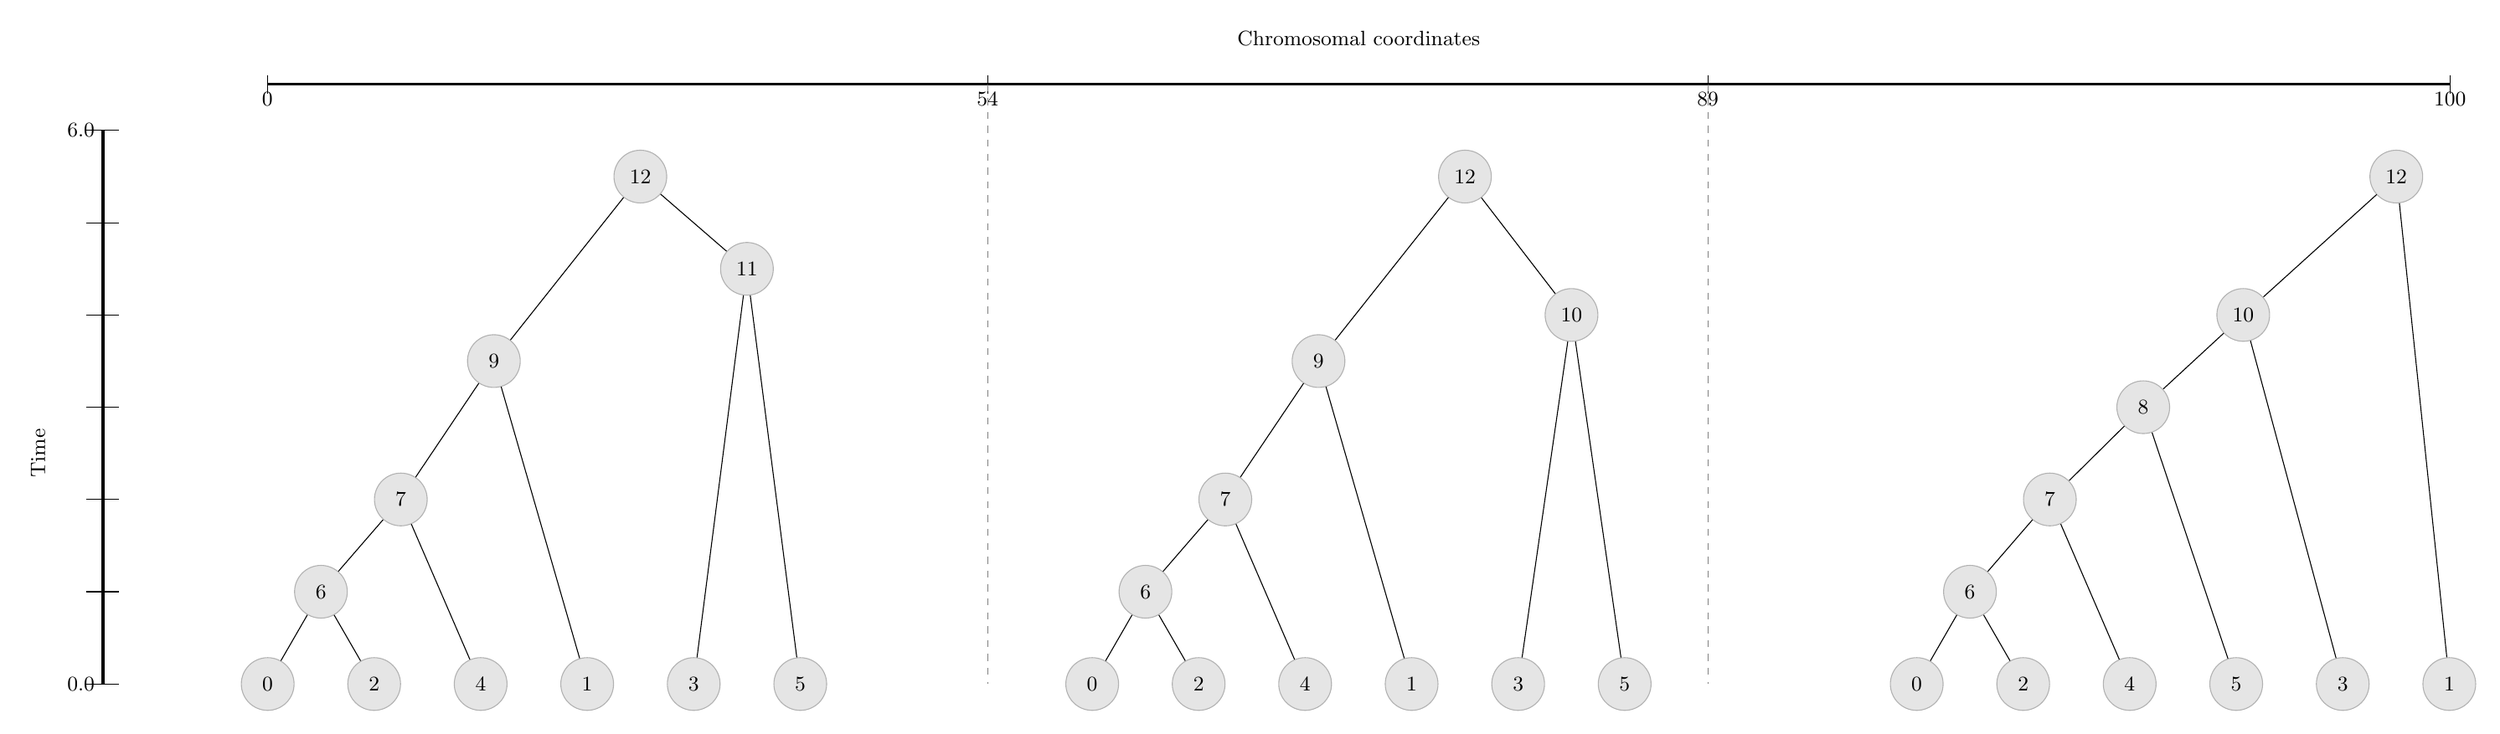
\begin{tikzpicture}[node distance=8mm and 8mm,xscale=2.5, yscale=1.4]

\tikzset{greynode/.style={font=\small,node distance=1cm and 1 cm,fill=black!10,draw=black!30,inner sep=0pt,minimum size=8mm,shape=circle},
mutations/.style={shape=starburst,fill=red!50!blue,inner sep=2pt,starburst points=11,starburst point height=.2cm}}

% Middle sample nodes
\node (s0) [greynode] {0};
\node (s2) [right=of s0,greynode] {2};
\node (s4) [right=of s2,greynode] {4};
\node (s1) [right=of s4,greynode] {1};
\node (s3) [right=of s1,greynode] {3};
\node (s5) [right=of s3,greynode] {5};

% Left sample nodes
\node (leftTree) at (-5, 0) {};
\node[greynode] (s0l) at ($(s0) + (leftTree)$) {0};
\node[greynode] (s1l) at ($(s1) + (leftTree)$) {1};
\node[greynode] (s2l) at ($(s2) + (leftTree)$) {2};
\node[greynode] (s3l) at ($(s3) + (leftTree)$) {3};
\node[greynode] (s4l) at ($(s4) + (leftTree)$) {4};
\node[greynode] (s5l) at ($(s5) + (leftTree)$) {5};

% Right sample nodes
\node (rightTree) at (5, 0) {};
\node[greynode] (s0r) at ($(s0) + (rightTree)$) {0};
\node[greynode] (s1r) at ($(s5) + (rightTree)$) {1};
\node[greynode] (s2r) at ($(s2) + (rightTree)$) {2};
\node[greynode] (s3r) at ($(s3) + (rightTree)$) {3};
\node[greynode] (s4r) at ($(s4) + (rightTree)$) {4};
\node[greynode] (s5r) at ($(s1) + (rightTree)$) {5};

% Non-sample nodes
\node [greynode] (s6) at ($0.5*(s0) + 0.5*(s2) + (0,1)$) {6};
\node [greynode] (s6l) at ($(s6) + (leftTree)$) {6};
\node [greynode] (s6r) at ($(s6) + (rightTree)$) {6};

\node [greynode] (s7) at ($0.5*(s6) + 0.5*(s4) + (0, 1.5)$) {7};
\node [greynode] (s7l) at ($(s7) + (leftTree)$) {7};
\node [greynode] (s7r) at ($(s7) + (rightTree)$) {7};

\node [greynode] (s8r) at ($0.5*(s7r) + 0.5*(s5r) + (0,2) $) {8};

\node [greynode] (s9) at ($0.5*(s7) + 0.5*(s1) + (0,2.5)$) {9};
\node [greynode] (s9l) at ($0.5*(s7l) + 0.5*(s1l) + (0,2.5)$) {9};

\node [greynode] (s10) at ($0.5*(s3) + 0.5*(s5) + (0,4)$) {10};
\node [greynode] (s10r) at ($0.5*(s8r) + 0.5*(s3r) + (0,2.5)$) {10};

\node [greynode] (s11l) at ($0.5*(s3l) + 0.5*(s5l) + (0, 4.5)$) {11};

\node [greynode] (s12) at ($0.5*(s1) + 0.5*(s3) + (0,5.5)$) {12};
\node [greynode] (s12l) at ($0.5*(s1l) + 0.5*(s3l) + (0,5.5)$) {12};
\node [greynode] (s12r) at ($0.5*(s1r) + 0.5*(s3r) + (0,5.5)$) {12};

% Edges 
\draw (s0) -- (s6) -- (s2); \draw (s0l) -- (s6l) -- (s2l); \draw (s0r) -- (s6r) -- (s2r);
\draw (s6) -- (s7) -- (s4); \draw (s6l) -- (s7l) -- (s4l); \draw (s6r) -- (s7r) -- (s4r);
\draw (s7r) -- (s8r) -- (s5r);
\draw (s7) -- (s9) -- (s1); \draw (s7l) -- (s9l) -- (s1l);
\draw (s3) -- (s10) -- (s5); \draw (s8r) -- (s10r) -- (s3r);
\draw (s3l) -- (s11l) -- (s5l);
\draw (s9l) --(s12l) -- (s11l); \draw (s9) -- (s12) -- (s10); \draw (s10r) -- (s12r) -- (s1r);

% Axes
\node (leftAx) at (-6,0) {};
\draw[very thick] (-6,0) -- +(0, 6);
\foreach \y in {0, 1, 2, 3, 4, 5, 6} \draw ($(leftAx) + (-0.1, \y)$) -- ($(leftAx) + (0.1, \y)$); % tick marks
\draw[very thick] ($(s0l) + (0,6.5)$) -- ($(s1r) + (0,6.5)$);
\node (topAx) at (0,6.5) {};
\node (topLeft) at ($(s0l) + (0,6.5)$) {};
\node (genUnit) at ($0.1*(s1r) - 0.1*(s0l)$) {};
\foreach \x in {0, 3.3, 6.6, 10} \draw ($(topLeft) + \x*(genUnit) + (0,0.1)$) -- +(0, -0.2);
\node[anchor=east] at ($(leftAx)$) {\small 0.0}; \node[anchor=east] at ($(leftAx) + (0,6)$) {\small 6.0};
\node[anchor=north] at ($(topLeft)$) {\small 0};
\node[anchor=north] at ($(topLeft) + 3.3*(genUnit)$) {\small 54};
\node[anchor=north] at ($(topLeft) + 6.6*(genUnit)$) {\small 89};
\node[anchor=north] at ($(topLeft) + 10*(genUnit)$) {\small 100};

% Interval endpoints
\draw[thin,color=black!50,dashed] ($(topLeft) + 3.3*(genUnit)$) -- +(0, -6.5);
\draw[thin,color=black!50,dashed] ($(topLeft) + 6.6*(genUnit)$) -- +(0, -6.5);
%
%% Axis titles
\node (topLabel) at ($(topLeft) + 5*(genUnit) + (0,.5)$) {$\small\textrm{Chromosomal coordinates}$};
\node[rotate=90,anchor=south] (leftLabel) at ($(leftAx) + (-0.3,2.5)$) {$\small\textrm{Time}$};

% Mutations
%\node [mutations] (m1) at ($(s6l)!.5!(s7l)$) {};
%\node [mutations] (m1) at ($(s1r)!.3!(s8r)$) {};

\end{tikzpicture}

\end{center}
The algorithm returns the following IBD records for sample pair $(0, 5)$:
\[
\left( 89, 100; 8\right),
\left( 54, 89; 12\right),
\left( 0, 54; 12 \right)  
\]
You can make \texttt{find-ibd} more efficient by specifying a maximum age or minimum length for the IBD segments you're interested in. If \texttt{min-length=20}, the records are
\[
\left( 54, 89; 12\right),
\left( 0, 54; 12 \right)  
\]
If \texttt{max-time=50}, the only record is
\[
\left( 89, 100; 8\right)
\]
Since the IBD records contain information about the common ancestor, they can be dated to a particular time.
\texttt{find-ibd} requires a single pass over the edge table of the tree sequence, and each edge must only be processed once, regardless of how many gene trees it appears in.
This makes it extremely efficient.
          }           
       
\vspace{20cm}

             \block[titleoffsety=0cm,bodyoffsety=0cm]{Application 2: simulation-based inference}{

\begin{adjustbox}{valign=b}
\begin{minipage}[t]{0.5\linewidth}
{\small
\begin{tabularx}{.8\textwidth}{p{9cm}X}
\toprule
\multicolumn{2}{c}{\bf Model inference}\\
\midrule
Posterior probability for correct~model &  $96.33\% \pm 2.68\%$ \\
Votes for correct demography &$93.36\% \pm 4.69\%$\\
Prior error rate & $0.0993 \pm 0.0008$ \\
\bottomrule
\end{tabularx}
}
\end{minipage}\end{adjustbox}\begin{adjustbox}{valign=c}
\begin{minipage}[t]{0.35\linewidth}
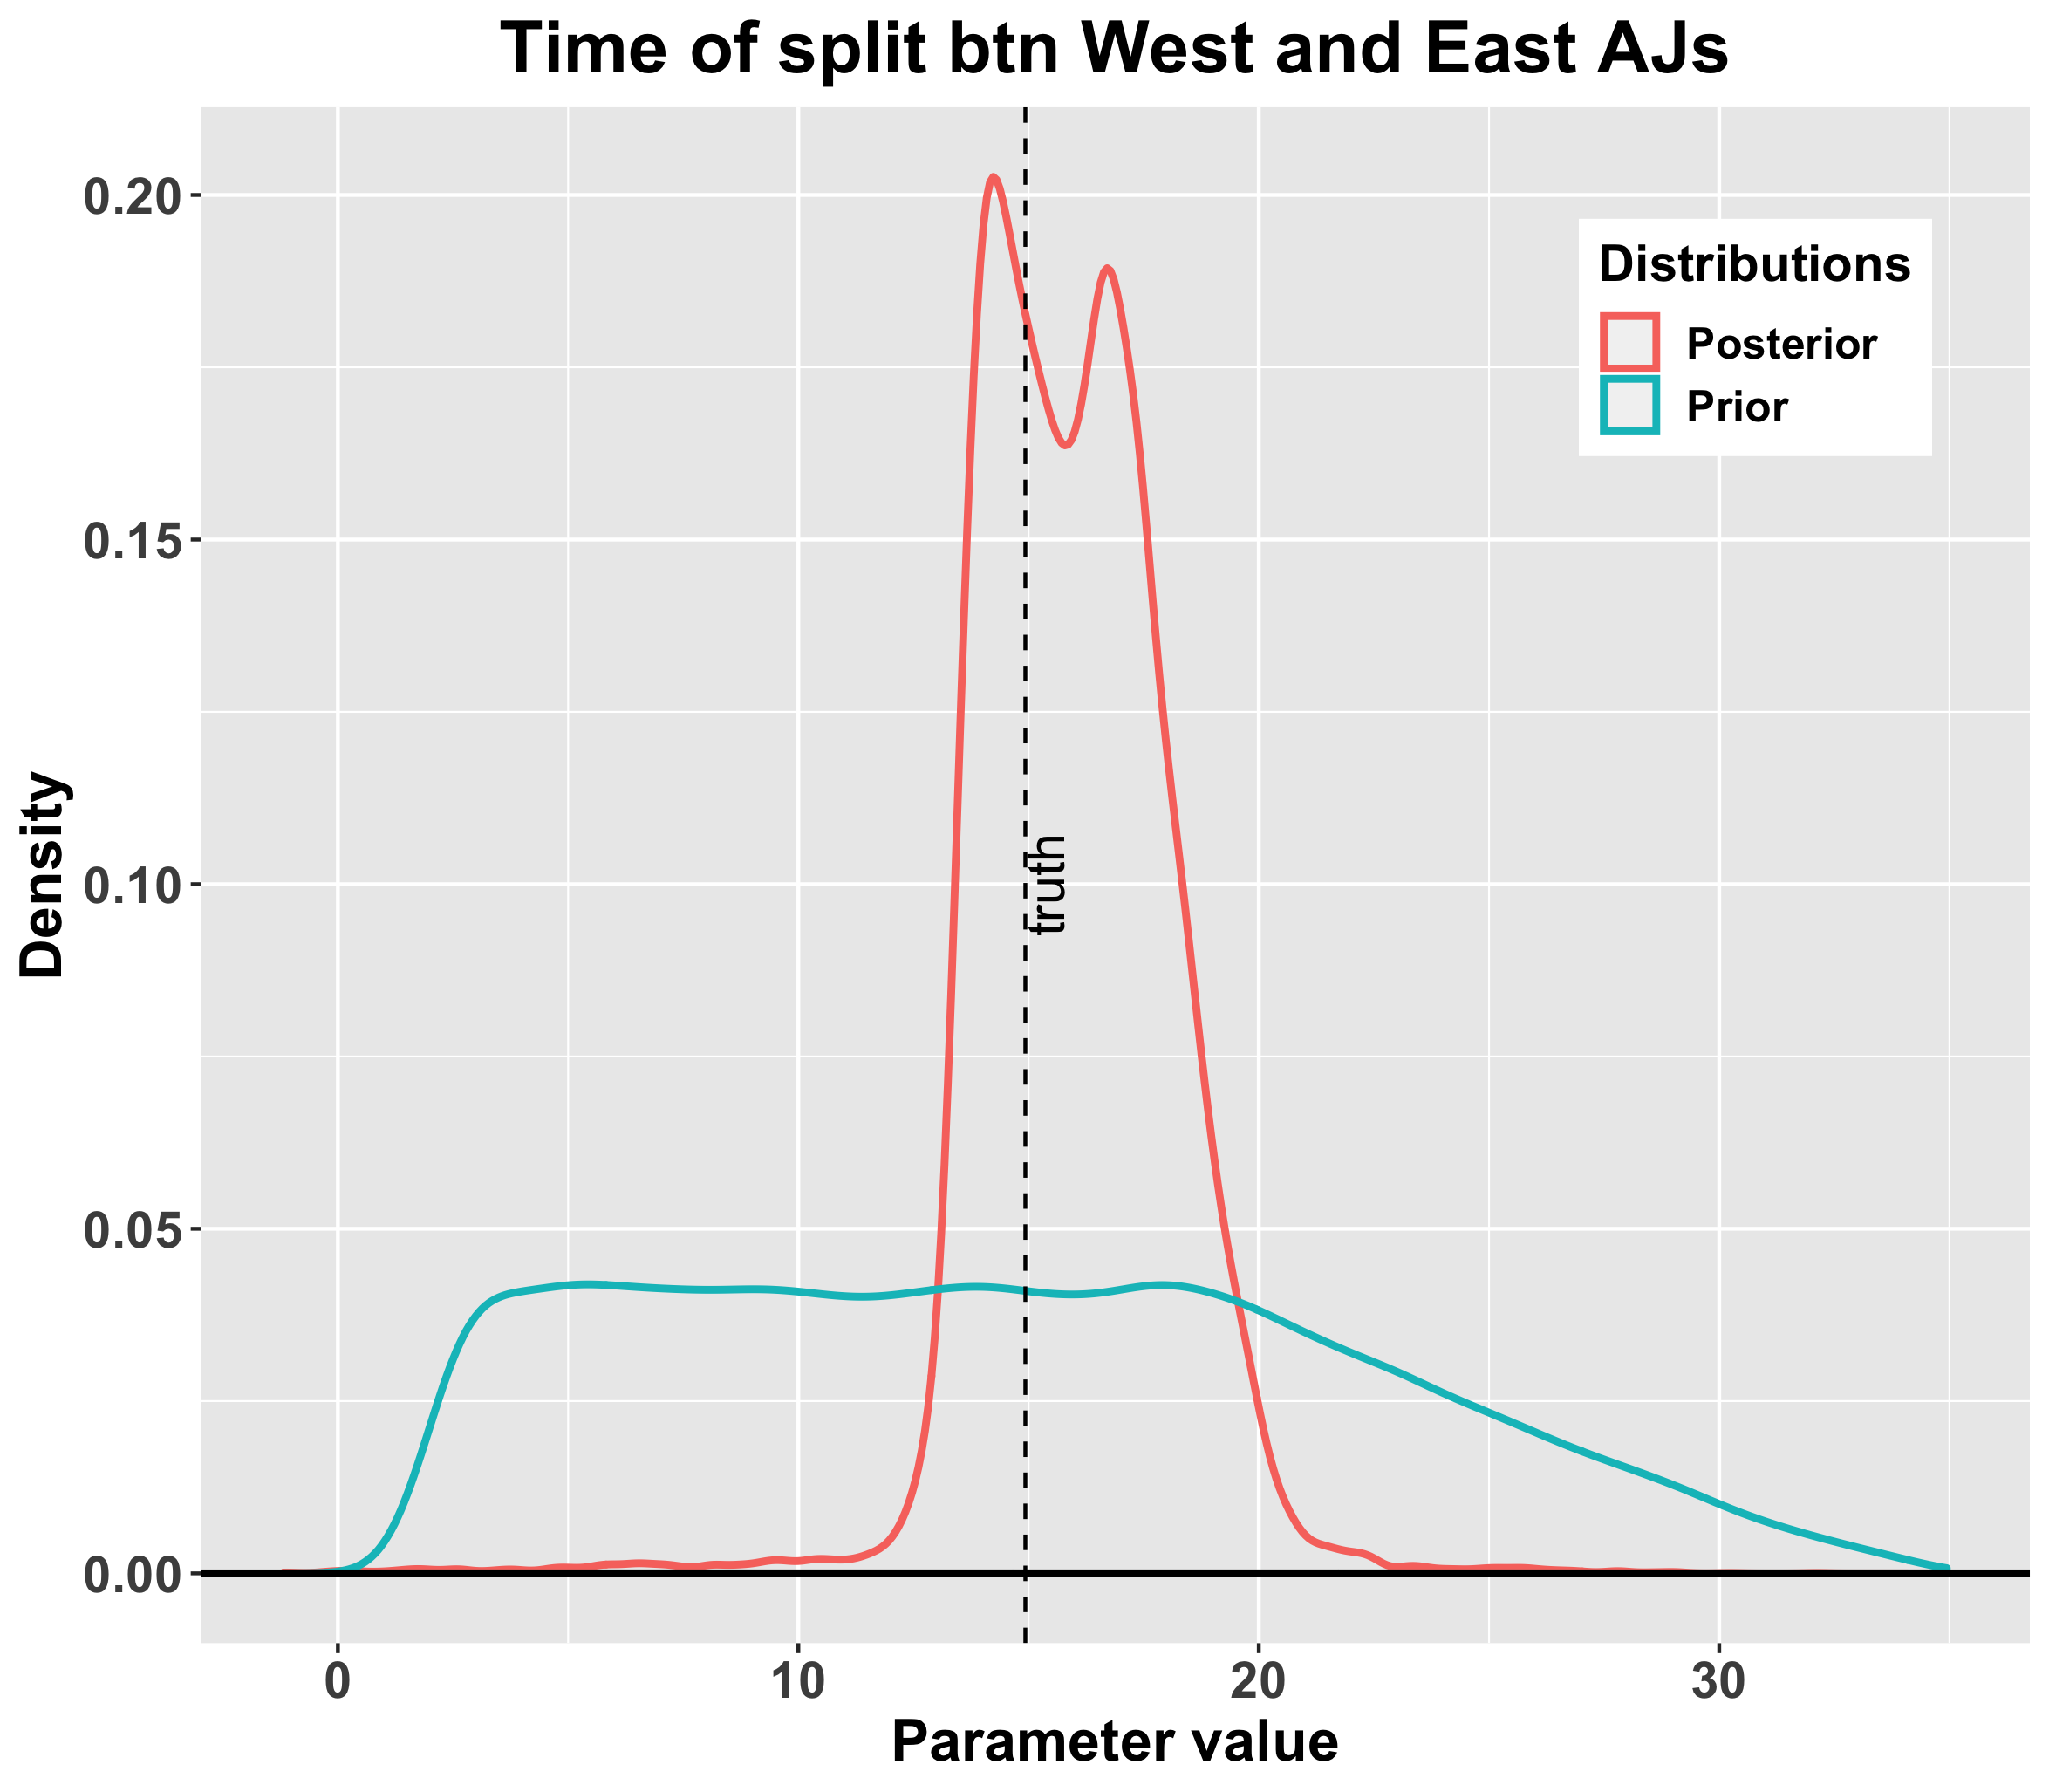
\includegraphics[scale=.2]{pics/abc-ibd-4.png}
\end{minipage}
\end{adjustbox}

{\fontsize{34}{35}\selectfont To explore the power of \texttt{find-ibd}, we used it to recreate some of the important findings from a recent study of Ashkenazi Jewish (AJ) demographic history [3]. This work provided evidence for a recent divergence event between Eastern and Western communities of AJ people. It was estimated that this happened about 15 generations ago.\\[2mm]
Closely following [3], we performed 100 000 simulations of various demographic scenarios with \texttt{msprime} [2], and 20 simulations under the parameter values inferred by [3], which we treated as artificial truth datasets. For each simulation, we calculated moments of IBD segment lengths at multiple time points. We used the \texttt{abcrf} package [4] to infer the most plausible demographic scenario, and the \texttt{abc} package [5] with neural-net regression to estimate parameter values.\\
All simulations and analyses ran on a standard desktop in $<12$ hours.
}
}
     \end{columns}

%%% BLOCK 5
 \block[titleoffsety=1.2cm,bodyoffsety=1.2cm]{5. Acknowledgements, references and further information}{
 }
  \begin{columns}
 \begin{subcolumns}
 \renewcommand\baselinestretch{1}\selectfont
    \subcolumn{22} \block[bodyoffsetx=1.5cm,bodyverticalshift=-5cm]{}{\footnotesize
     GT is funded by the Helen Freeman scholarship, the Maurice Belz Fund and the Australian Government's Research Training Scheme.\\[1mm]
     [1] \texttt{https://tskit.readthedocs.io/en/latest/}\\[1mm]
     [2] Kelleher, J., et al. (2016). Efficient Coalescent Simulation and Genealogical Analysis for Large Sample Sizes. PLOS Computational Biology, 12(5).\\[1mm]
     [3] Gladstein, A and Hammer, M. (2019). Substructured Population Growth in the Ashkenazi Jews Inferred with Approximate Bayesian Computation. Molecular Biology and Evolution, 36(6), 1162-1171.\\[1mm] 
    [4] Raynal, L., et al. (2019). ABC random forests for Bayesian parameter inference. Bioinformatics, 35(10), 1720 - 1728.\\[1mm]
	[5] Csillery, K., et al. (2012). Abc: An R package for approximate Bayesian computation (ABC). Methods in Ecology and Evolution, 3(3), 475 - 479.\\[1mm]
	[6] Wohns, A. W., et al. (2021). A unified genealogy of modern and ancient genomes, 1–31. https://doi.org/10.1101/2021.02.16.431497\\[1mm]
	[7] Bergström, A.,et al. (2020). Insights into human genetic variation and population history from 929 diverse genomes. Science, 367(6484). https://doi.org/10.1126/science.aay5012
     }

       \subcolumn{3} \block[bodyoffsetx=-3cm,bodyverticalshift=-5.7cm]{}{
       \begin{center}
       {\small Come say hi!}\\
       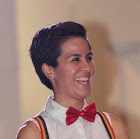
\includegraphics[scale=1]{pics/GT_headshot.jpg} 
       \end{center}
       }
       \subcolumn{3} \block[bodyoffsetx=-4cm,bodyverticalshift=-5cm]{}{
       \begin{center}
       
\includegraphics[scale=1.2]{pics/unimelb-logo.jpg}
      \end{center}
       }
       \subcolumn{3} \block[bodyoffsetx=-5cm,bodyverticalshift=-6cm]{}{
       \begin{center}
       
\includegraphics[scale=1]{pics/tskit-logo.png}
      \end{center}
       }
 \end{subcolumns}
 \end{columns}         

 \end{document}


\endinput
%%
%% End of file `tikzposter-example.tex'.
